\chapter{Anhang}
\label{chapter:anhang}


\begin{figure}
		\centering
		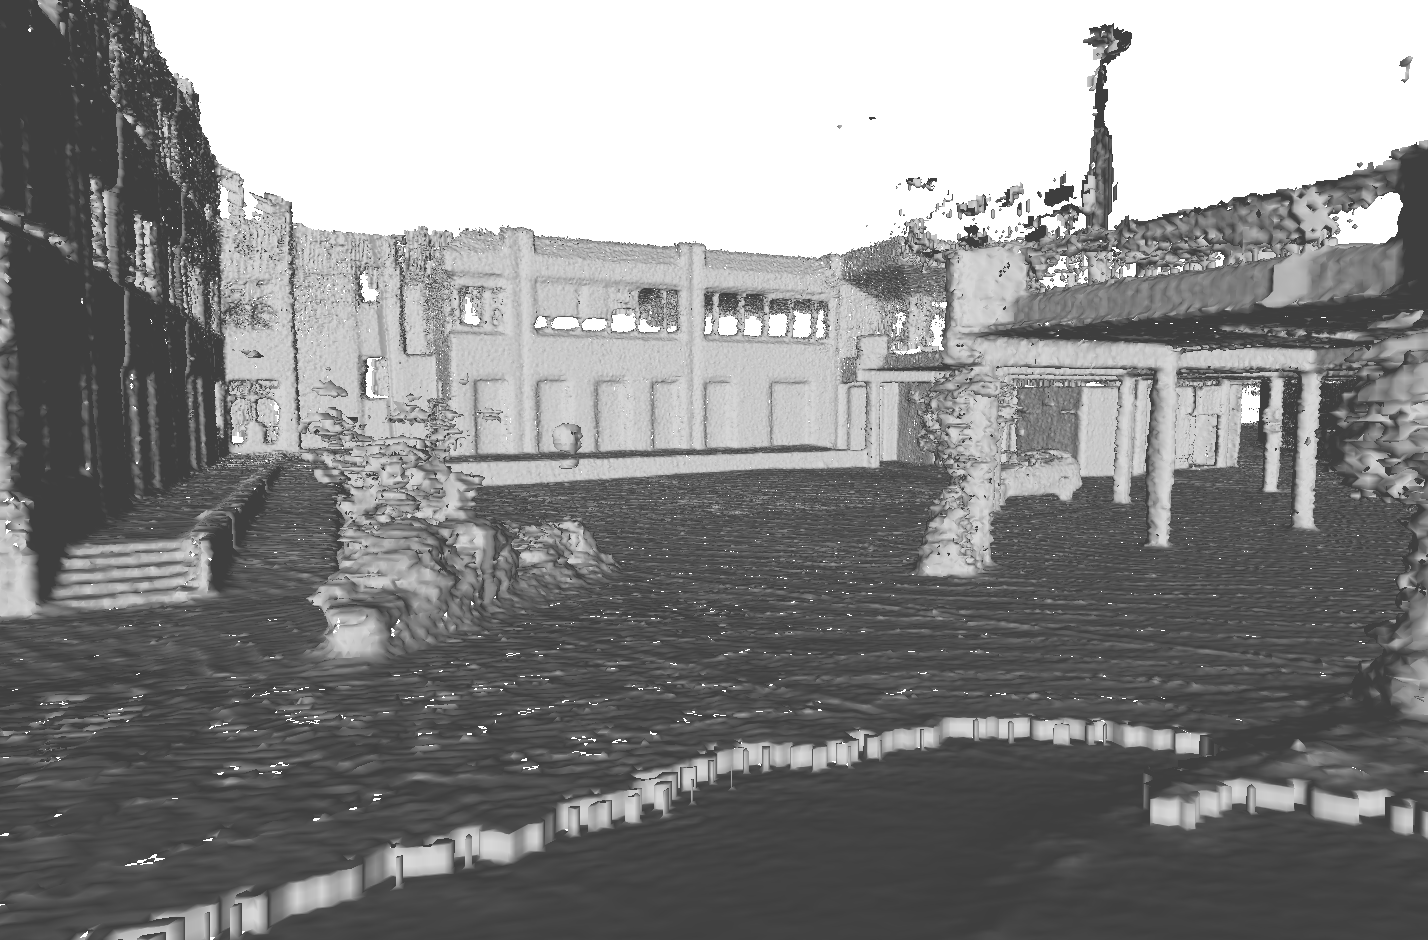
\includegraphics
			[scale=0.5, angle=90]
			{physik_unten_mesh}
		\caption
			[Caption for LOF]{\emph{Marching-Cubes}-Rekonstruktion \cite{lorensen_marching_1987} des in Kapitel \ref{chapter:loop_closure} vorgestellten Datensatzes des Physikgebäudes der Universität Osnabrück. In einem Nachbearbeitungsschritt wurden Löcher im Mesh geschlossen und eine Glättung durchgeführt.}                                                                                                                                     
		\label{fig:mesh_phsysik_unten}
\end{figure}


\begin{figure}
		\centering
		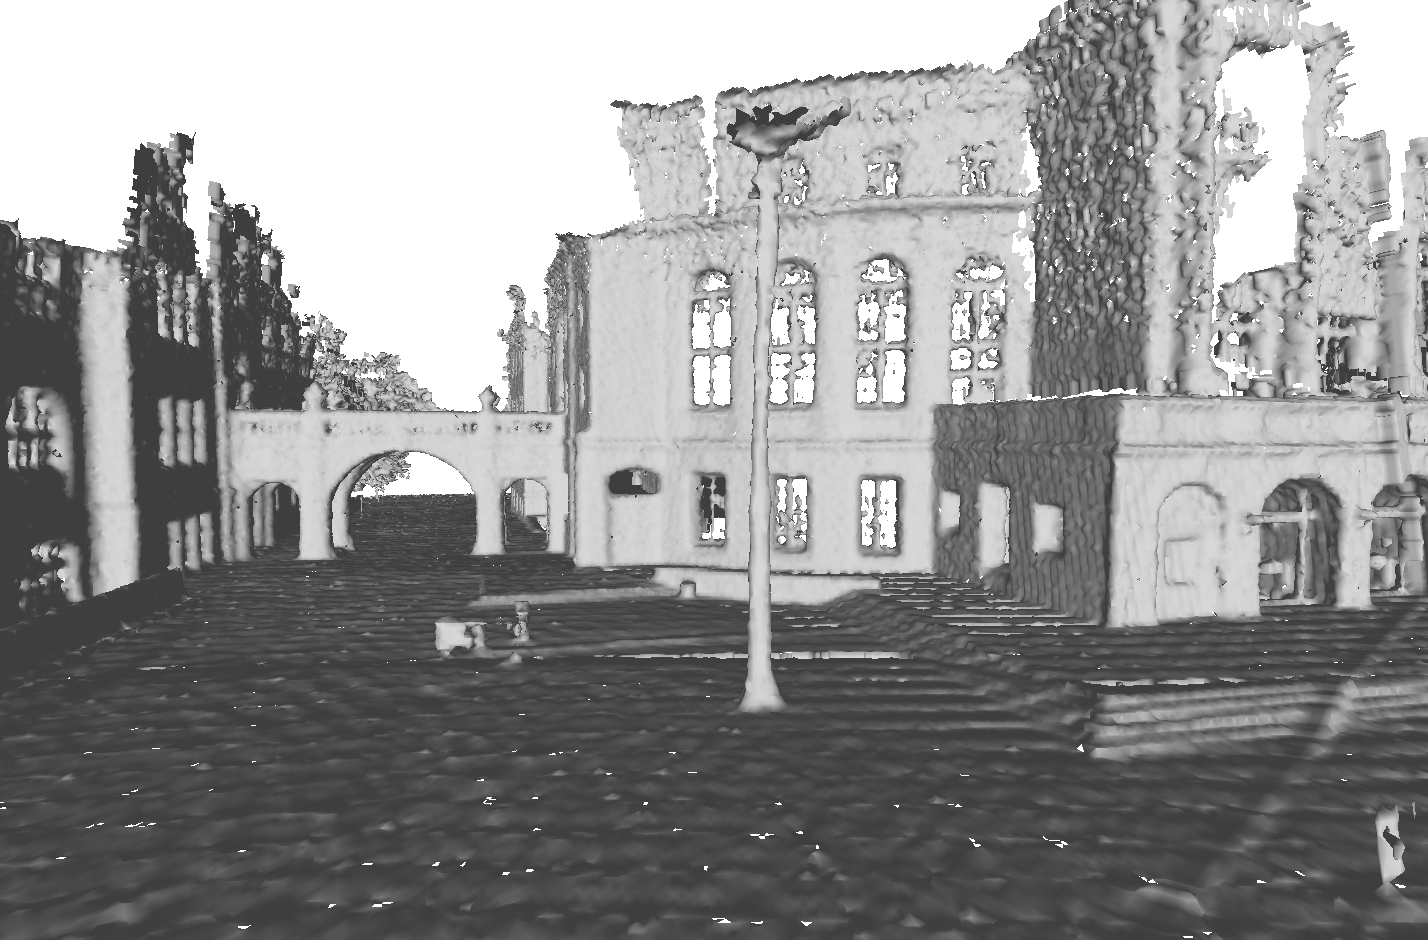
\includegraphics
			[scale=0.5, angle=90]
			{mesh_vorplatz_1}
		\caption
			[Caption for LOF]{\emph{Marching-Cubes}-Rekonstruktion \cite{lorensen_marching_1987} des in Kapitel \ref{chapter:loop_closure} vorgestellten Datensatzes des Chemnitzer Opernhauses. In einem Nachbearbeitungsschritt wurden Löcher im Mesh geschlossen und eine Glättung durchgeführt.}                                                                                                                                     
		\label{fig:mesh_vorplatz_1}
\end{figure}


\begin{figure}
		\centering
		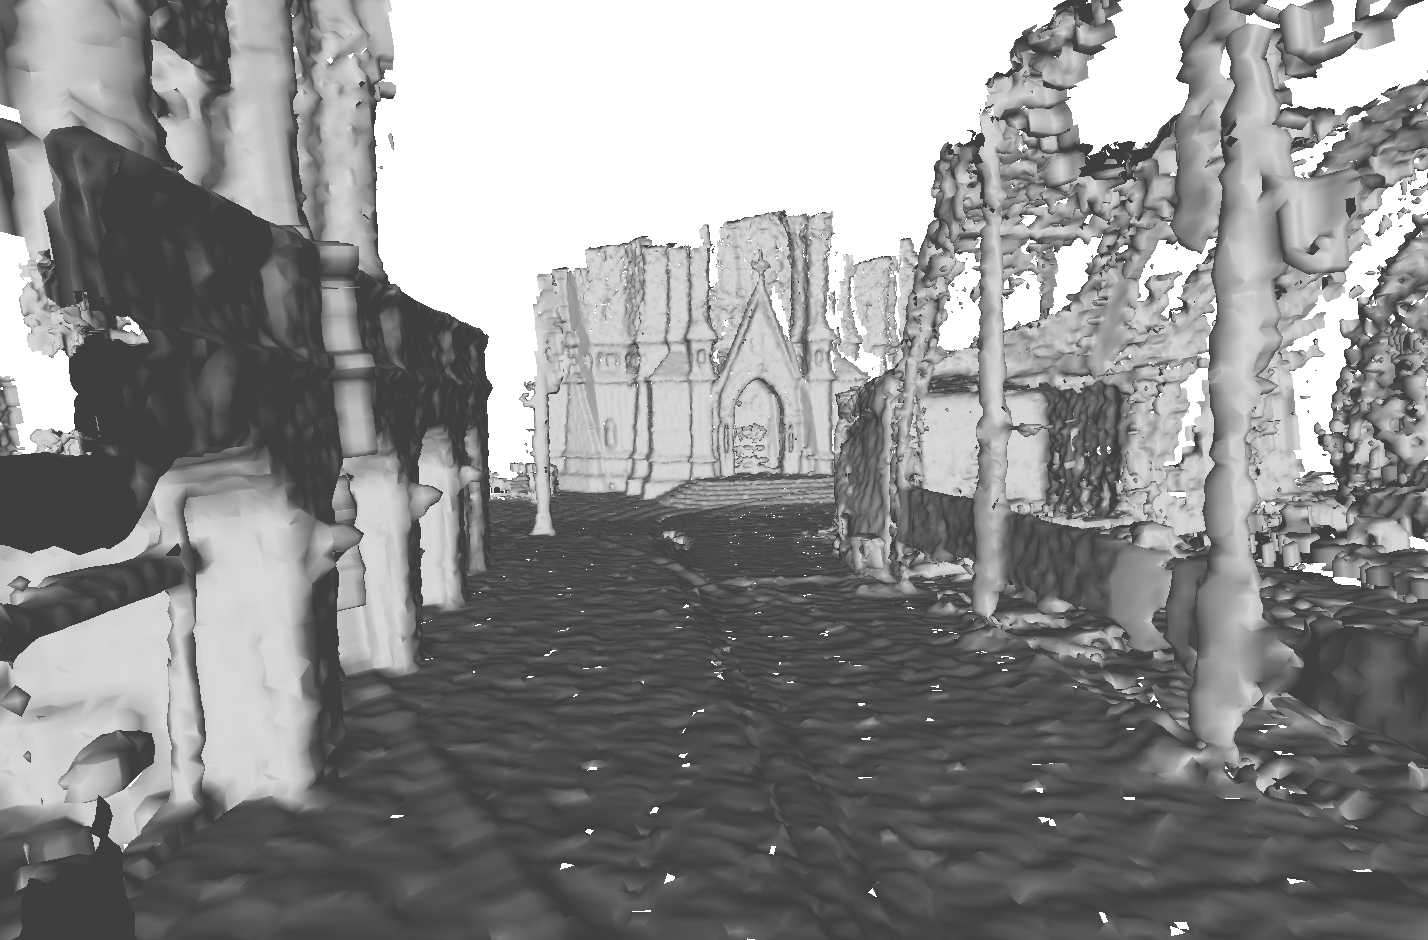
\includegraphics
			[scale=0.5, angle=90]
			{mesh_vorplatz_2}
		\caption
			[Caption for LOF]{\emph{Marching-Cubes}-Rekonstruktion \cite{lorensen_marching_1987} des in Kapitel \ref{chapter:loop_closure} vorgestellten Datensatzes des Physikgebäudes der Universität Osnabrück. In einem Nachbearbeitungsschritt wurden Löcher im Mesh geschlossen und eine Glättung durchgeführt.}                                                                                                                                     
		\label{fig:mesh_vorplatz_2}
\end{figure}

\begin{figure}
		\centering
		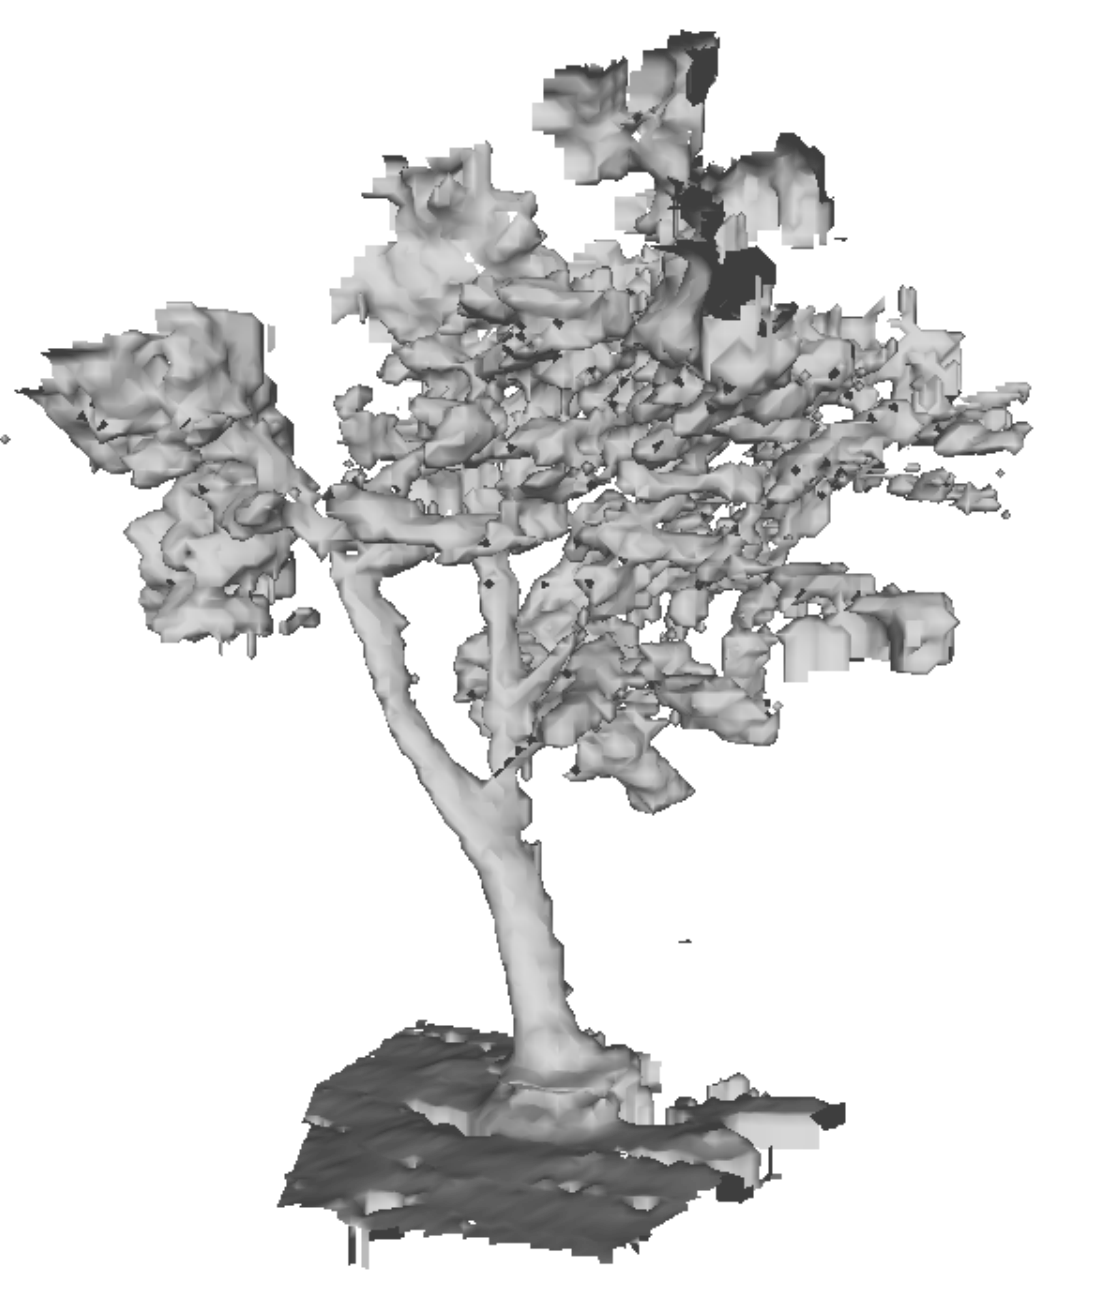
\includegraphics
			[scale=1.1]
			{mesh_tree}
		\caption
			[Caption for LOF]{Dreiecksnetz entnommen aus dem Netz aus Abbildung \ref{fig:mesh_vorplatz_1}. Zu sehen ist ein Baum des Datensatzes des Vorplatzes des Chemnitzer Opernhauses. Die zugrunde liegende TSDF-Karte hat eine Auflösung von $124mm$. Trotz der geringen Auflösung der Karte sind hier deutlich die Teilstrukturen des Baumes zu erkennen. Dies spricht für eine exakte Pose-Bestimmung. }                                                                                                                                     
		\label{fig:mesh_tree}
\end{figure}